% Generated by LitigCharts.PublicationFigures. Captions and provenance are sidecars.
\documentclass[10pt,tikz,border=5pt]{standalone}
\usepackage{lmodern}
\usetikzlibrary{patterns,patterns.meta}
\begin{document}
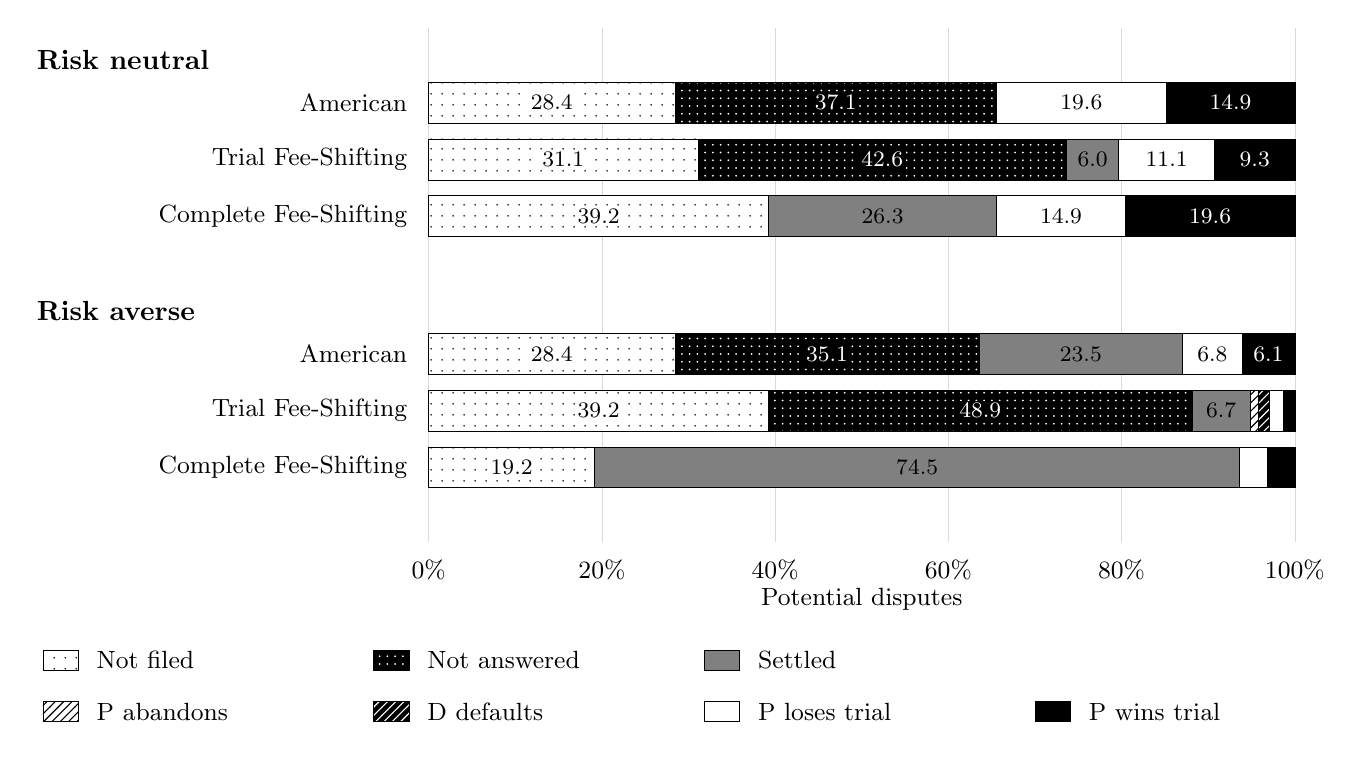
\begin{tikzpicture}[font=\small]\draw[black!15,line width=.2pt] (5.1,.65) -- (5.1,7.18);
\node[anchor=north] at (5.1,.55) {0\%};
\draw[black!15,line width=.2pt] (7.3,.65) -- (7.3,7.18);
\node[anchor=north] at (7.3,.55) {20\%};
\draw[black!15,line width=.2pt] (9.5,.65) -- (9.5,7.18);
\node[anchor=north] at (9.5,.55) {40\%};
\draw[black!15,line width=.2pt] (11.7,.65) -- (11.7,7.18);
\node[anchor=north] at (11.7,.55) {60\%};
\draw[black!15,line width=.2pt] (13.9,.65) -- (13.9,7.18);
\node[anchor=north] at (13.9,.55) {80\%};
\draw[black!15,line width=.2pt] (16.1,.65) -- (16.1,7.18);
\node[anchor=north] at (16.1,.55) {100\%};
\node[anchor=west,font=\bfseries] at (0,6.78) {\mbox{Risk} \mbox{neutral}};
\node[anchor=east] at (4.95,6.23) {American};
\path[preaction={fill=white,draw=none},pattern={Dots[distance=4pt,radius=.35pt]},pattern color=black,draw=black,line width=.25pt] (5.1,5.97) rectangle (8.22741,6.49);
\node[text=black,fill=white,font=\footnotesize,inner sep=1pt] at (6.663705,6.23) {28.4};
\path[preaction={fill=black,draw=none},pattern={Dots[distance=2.8pt,radius=.35pt]},pattern color=white,draw=black,line width=.25pt] (8.22741,5.97) rectangle (12.312766,6.49);
\node[text=white,fill=black,font=\footnotesize,inner sep=1pt] at (10.270088,6.23) {37.1};
\path[fill=white,draw=black,line width=.25pt] (12.312766,5.97) rectangle (14.464685,6.49);
\node[text=black,fill=none,font=\footnotesize,inner sep=1pt] at (13.388726,6.23) {19.6};
\path[fill=black,draw=black,line width=.25pt] (14.464685,5.97) rectangle (16.1,6.49);
\node[text=white,fill=none,font=\footnotesize,inner sep=1pt] at (15.282343,6.23) {14.9};
\node[anchor=east] at (4.95,5.51) {Trial Fee-Shifting};
\path[preaction={fill=white,draw=none},pattern={Dots[distance=4pt,radius=.35pt]},pattern color=black,draw=black,line width=.25pt] (5.1,5.25) rectangle (8.518602,5.77);
\node[text=black,fill=white,font=\footnotesize,inner sep=1pt] at (6.809301,5.51) {31.1};
\path[preaction={fill=black,draw=none},pattern={Dots[distance=2.8pt,radius=.35pt]},pattern color=white,draw=black,line width=.25pt] (8.518602,5.25) rectangle (13.200312,5.77);
\node[text=white,fill=black,font=\footnotesize,inner sep=1pt] at (10.859457,5.51) {42.6};
\path[fill=black!50,draw=black,line width=.25pt] (13.200312,5.25) rectangle (13.861933,5.77);
\node[text=black,fill=none,font=\footnotesize,inner sep=1pt] at (13.531123,5.51) {6.0};
\path[fill=white,draw=black,line width=.25pt] (13.861933,5.25) rectangle (15.081976,5.77);
\node[text=black,fill=none,font=\footnotesize,inner sep=1pt] at (14.471955,5.51) {11.1};
\path[fill=black,draw=black,line width=.25pt] (15.081976,5.25) rectangle (16.100015,5.77);
\node[text=white,fill=none,font=\footnotesize,inner sep=1pt] at (15.590996,5.51) {9.3};
\node[anchor=east] at (4.95,4.79) {Complete Fee-Shifting};
\path[preaction={fill=white,draw=none},pattern={Dots[distance=4pt,radius=.35pt]},pattern color=black,draw=black,line width=.25pt] (5.1,4.53) rectangle (9.41651,5.05);
\node[text=black,fill=white,font=\footnotesize,inner sep=1pt] at (7.258255,4.79) {39.2};
\path[fill=black!50,draw=black,line width=.25pt] (9.41651,4.53) rectangle (12.312832,5.05);
\node[text=black,fill=none,font=\footnotesize,inner sep=1pt] at (10.864671,4.79) {26.3};
\path[fill=white,draw=black,line width=.25pt] (12.312832,4.53) rectangle (13.948147,5.05);
\node[text=black,fill=none,font=\footnotesize,inner sep=1pt] at (13.13049,4.79) {14.9};
\path[fill=black,draw=black,line width=.25pt] (13.948147,4.53) rectangle (16.1,5.05);
\node[text=white,fill=none,font=\footnotesize,inner sep=1pt] at (15.024074,4.79) {19.6};
\node[anchor=west,font=\bfseries] at (0,3.59) {\mbox{Risk} \mbox{averse}};
\node[anchor=east] at (4.95,3.04) {American};
\path[preaction={fill=white,draw=none},pattern={Dots[distance=4pt,radius=.35pt]},pattern color=black,draw=black,line width=.25pt] (5.1,2.78) rectangle (8.22741,3.3);
\node[text=black,fill=white,font=\footnotesize,inner sep=1pt] at (6.663705,3.04) {28.4};
\path[preaction={fill=black,draw=none},pattern={Dots[distance=2.8pt,radius=.35pt]},pattern color=white,draw=black,line width=.25pt] (8.22741,2.78) rectangle (12.087882,3.3);
\node[text=white,fill=black,font=\footnotesize,inner sep=1pt] at (10.157646,3.04) {35.1};
\path[fill=black!50,draw=black,line width=.25pt] (12.087882,2.78) rectangle (14.677524,3.3);
\node[text=black,fill=none,font=\footnotesize,inner sep=1pt] at (13.382703,3.04) {23.5};
\path[fill=white,draw=black,line width=.25pt] (14.677524,2.78) rectangle (15.429095,3.3);
\node[text=black,fill=none,font=\footnotesize,inner sep=1pt] at (15.053309,3.04) {6.8};
\path[fill=black,draw=black,line width=.25pt] (15.429095,2.78) rectangle (16.10001,3.3);
\node[text=white,fill=none,font=\footnotesize,inner sep=1pt] at (15.764552,3.04) {6.1};
\node[anchor=east] at (4.95,2.32) {Trial Fee-Shifting};
\path[preaction={fill=white,draw=none},pattern={Dots[distance=4pt,radius=.35pt]},pattern color=black,draw=black,line width=.25pt] (5.1,2.06) rectangle (9.41651,2.58);
\node[text=black,fill=white,font=\footnotesize,inner sep=1pt] at (7.258255,2.32) {39.2};
\path[preaction={fill=black,draw=none},pattern={Dots[distance=2.8pt,radius=.35pt]},pattern color=white,draw=black,line width=.25pt] (9.41651,2.06) rectangle (14.794872,2.58);
\node[text=white,fill=black,font=\footnotesize,inner sep=1pt] at (12.105691,2.32) {48.9};
\path[fill=black!50,draw=black,line width=.25pt] (14.794872,2.06) rectangle (15.533317,2.58);
\node[text=black,fill=none,font=\footnotesize,inner sep=1pt] at (15.164095,2.32) {6.7};
\path[preaction={fill=white,draw=none},pattern={north east lines},pattern color=black,draw=black,line width=.25pt] (15.533317,2.06) rectangle (15.63622,2.58);
\path[preaction={fill=black,draw=none},pattern={north east lines},pattern color=white,draw=black,line width=.25pt] (15.63622,2.06) rectangle (15.775155,2.58);
\path[fill=white,draw=black,line width=.25pt] (15.775155,2.06) rectangle (15.947621,2.58);
\path[fill=black,draw=black,line width=.25pt] (15.947621,2.06) rectangle (16.100005,2.58);
\node[anchor=east] at (4.95,1.6) {Complete Fee-Shifting};
\path[preaction={fill=white,draw=none},pattern={Dots[distance=4pt,radius=.35pt]},pattern color=black,draw=black,line width=.25pt] (5.1,1.34) rectangle (7.20672,1.86);
\node[text=black,fill=white,font=\footnotesize,inner sep=1pt] at (6.15336,1.6) {19.2};
\path[fill=black!50,draw=black,line width=.25pt] (7.20672,1.34) rectangle (15.400026,1.86);
\node[text=black,fill=none,font=\footnotesize,inner sep=1pt] at (11.303373,1.6) {74.5};
\path[fill=white,draw=black,line width=.25pt] (15.400026,1.34) rectangle (15.74997,1.86);
\path[fill=black,draw=black,line width=.25pt] (15.74997,1.34) rectangle (16.100001,1.86);
\node at (10.6,-.08) {Potential disputes};
\path[preaction={fill=white,draw=none},pattern={Dots[distance=4pt,radius=.35pt]},pattern color=black,draw=black,line width=.25pt] (0.2,-0.98) rectangle (0.65,-0.72);
\node[anchor=west] at (0.76,-0.85) {Not filed};
\path[preaction={fill=black,draw=none},pattern={Dots[distance=2.8pt,radius=.35pt]},pattern color=white,draw=black,line width=.25pt] (4.4,-0.98) rectangle (4.85,-0.72);
\node[anchor=west] at (4.96,-0.85) {Not answered};
\path[fill=black!50,draw=black,line width=.25pt] (8.6,-0.98) rectangle (9.05,-0.72);
\node[anchor=west] at (9.16,-0.85) {Settled};
\path[preaction={fill=white,draw=none},pattern={north east lines},pattern color=black,draw=black,line width=.25pt] (0.2,-1.63) rectangle (0.65,-1.37);
\node[anchor=west] at (0.76,-1.5) {P abandons};
\path[preaction={fill=black,draw=none},pattern={north east lines},pattern color=white,draw=black,line width=.25pt] (4.4,-1.63) rectangle (4.85,-1.37);
\node[anchor=west] at (4.96,-1.5) {D defaults};
\path[fill=white,draw=black,line width=.25pt] (8.6,-1.63) rectangle (9.05,-1.37);
\node[anchor=west] at (9.16,-1.5) {P loses trial};
\path[fill=black,draw=black,line width=.25pt] (12.8,-1.63) rectangle (13.25,-1.37);
\node[anchor=west] at (13.36,-1.5) {P wins trial};
\end{tikzpicture}
\end{document}
